\chapter{Análise Bibliográfica sobre Análise de Dados integradas em Nuvem para auxílio de Fenômenos Sociais, por Guilherme Oliveira Loiola\label{chap:bibliometria:guioliunb}}

\section{Planejamento do estudo\label{MASSA:coleta}}
O planejamento o  desenho do estudo deve descrever as motivações, questões de interesse, escopo, limitações e objetivos do trabalho.

O planejamento do estudo deve motivar o tema escolhido e o interesse do autor.

No caso do meu trabalho, as perguntas que o nortearam foram:
\begin{itemize}
    \item Qual a base de conhecimentos científicos produzida com análises de dados com auxílio da computação em nuvem voltada à compreensão de fenômenos sociais? 
    \item Como a capacidade de processamento da nuvem está proporcionando análises sociais mais precisas e eficientes? 
    \item Quais são as principais aplicações de interesse da comunidade científica diante da evolução tecnológica dos últimos anos?
    \item Quais os principais métodos de análise e ferramentas de aplicação nos problemas atuais?
\end{itemize}

\subsection{O que já existe de pesquisa bibliométrica sobre esse tema?}

\cite{ma_method_2020} realizou uma pesquisa que visava combinar a capacidade de processamento da computação em nuvem com os algoritmos de inteligência artificial para auxiliar na identificação de padrões e criação de metodologias de tratamento para dificuldades enfrentadas na psiquiatria.

Assim como \cite{archenaa_interactive_2016} que promoveu um estudo enfrentando desafios da saúde utilizando computação em nuvem (utilizando a tecnologia \textit{Apache Spark}).


\subsection{Uso do Bibliometrix e Biblioshiny}
Serão usadas a ferramenta e o \textit{workflow} proposto pelos autores do pacote Bibliometrix.

\subsection{Limitações} O exercício relatado foi feito em uma semana, envolvendo de um autor. As bases de dados foram buscadas na plataforma WoS,


\section{Coleta de dados\label{MASSA:coleta}}

A coleta de dados feita usando o WoS no dia 08 de janeiro de 2022, acessado por meio do Portal de Periódicos da CAPES.

Foram feitas buscas na coleções \textbf{Web of Science - Coleção Principal (Clarivate Analytics) } que possui uma vasta bibliografia sobre a área de tecnologia. Através do refinamento nessa grande base foi obtido a base de dados composta por duas \query\ de pesquisa. A primeira coleta é mais simples com as palavras de maior relevância. Já a segunda, inclui alguns termos mais abrangentes e ponderando mais a questão de influência na sociedade. 

Ao todo foi agrupado um total de 2906 registros para a análise bibliométrica. Sendo 1000 registros originados da primeira \query\ e a segunda query contando com 1906 registros.

Além disso, foi realizado um refinamento das \query\ originais para eliminar algumas categorias de registros que fugiam do interesse do estudo. Temos os filtros: de linguagem para inglês (linguagem amplamente utilizada), restrição para o período de 2014 até 2022, documentos do tipo artigo/artigo de conferência e áreas de pesquisa ligadas à computação, engenharia e telecomunicações.

\subsection{Query de Busca}

Foram utilizadas duas \query\ de busca que estão ilustradas a seguir: %\ref{fig:}.

\lstinputlisting[numbers=left,basicstyle=\normalsize\ttfamily,caption={\query\  de busca sobre análises de dados que utilizam computação em nuvem para impactar a sociedade positivamente},label=query20210803-2]
{experiments/guioliunb/AnaliseBibliometrica/SocialBigDataAnalysis/WoS-dataset1/query1.txt}

\lstinputlisting[numbers=left,basicstyle=\normalsize\ttfamily,caption={\query\  de busca sobre análises de dados que utilizam computação em nuvem para impactar a sociedade positivamente},label=query1002]
{experiments/guioliunb/AnaliseBibliometrica/SocialBigDataAnalysis/WoS-dataset2/query2.txt}

\subsubsection{Explicação para os termos de busca usados\label{MASSA:query}}

As \query\ utilizadas foram criadas com intuitos semelhantes. A primeira mais restrita pelas palavras-chaves ligadas com tecnologia e separando a expressão de \texttt{big data} em \texttt{big} e \texttt{data} podendo ser duas possibilidades de ocorrência nos artigos. E a segunda \query\ reforça o intuito que a pesquisa tenha aplicação social e possibilitando também que o assunto  \texttt{database} ingresse ao conjunto.

A busca consistiu basicamente de quatro principais assuntos (\textit{Big Data}, \textit{Cloud}, \textit{Analytics}, \textit{Social}) aplicados à busca por tópico (O termo de busca pode aparecer no Título, no Abstract, na Author Keywords, ou nas Keywords Plus da referência).

Com a intersecção das áreas de competência sendo filtradas pela pesquisa de registros, juntamente, na união dos conjuntos de registros de ambas \query\ obtivemos artigos que focavam bem no assunto proposto.

\subsection{Registros recuperados}

Os 2.906 registros obtidos como resultado da busca encontram-se no projeto Overleaf da ferramenta utilizada na tarefa Computação Experimental - Turma A em \url{https://www.overleaf.com/project/618e9b4b0db7234d6d9fbfc0} . 

Foram utilizadas as opções \textit{Exportar registros para arquivo de texto sem formatação} e \textit{export full record / Gravar Conteúdo: Seleção personalizada, com todos os 29 campos disponíveis, inclusive referências citadas} no WoS, para que as citações também fosse usadas em análises da citações (estrutura intelectual do conhecimento). Os 2906 registros foram recuperados em dois blocos com mil registros da primeira consulta (1000) e quatro blocos da segunda consulta (2906), assim totalizando os 2906 registro  separados de até 500 registros por vez (1-500, 501-1000, 1001-1500, 1501-2000, ...).

A listagem \ref{record20210803-2} apresenta as 66 linhas de um registro no formato RIS, referentes a um artigo recuperado da Web of Science. Cada um dos campos de um registro é marcado por um código de dois caracteres, nas colunas 1 e 2 de cada linha. Se a coluna está em branco repete-se o mesmo campo da linha anterior.

Alguns campos específicos serão comentados a seguir:
\begin{description}
    \item [PT - Publication Type] indica o tipo da publicação, no caso específico um artigo de \textit{journal} (J);
    \item [AU - Author] Nome de um autor;
    \item [AF - Author Full Name] Nome completo de um autor;
    \item [TI - Title] Título da publicação;
    \item [SO - Source] Nome da revista;
    \item [DE - Descriptor] Palavras-chave;
    \item [AB - Abstract] Resumo;
    \item [CR - Cited Referente] Cada uma das referências citadas no artigo;
    \item [TC - Times Cited] Quantidade de vezes que esse artigo foi globalmente citado;
    \item [PY - Publication Year] Ano de publicação;
    \item [VL - Volume, IS - Issue] Volume e número onde o artigo foi publicado, na revista;
    \item [BP - Begin page, EP - End page] Páginas inicial e final do artigo dentro do volume e número da revista;
    \item [DI - Digital Object Identifier] Identificador único do artigo no sistema \url{http://doi.org};
    \item [DA - Date of Acquisition] Data em que o registro foi obtido da WoS;
    \item [ER - End of Record] Fim do registro.
\end{description}

\lstinputlisting[language={},numbers=left,basicstyle=\tiny\ttfamily,caption={Exemplo de um registro recuperado no formato RIS, sobre o tema Cloud-based Big Data Analysis},label=record20210803-2]
{experiments/guioliunb/AnaliseBibliometrica/SocialBigDataAnalysis/record.txt}

\section{Análise dos dados}

\subsection{Filtragem de registros}
Antes da análise, é possível aplicar filtros sobre os registros obtidos. Anteriormente, a primeira buscava contava com 1.343 registros e a segunda com 3.360 registros. Em ambas foi aplicado a mesma combinação de registros.

Foi aplicado um filtro ao \dataset\ inicial, com 4.703 registros, que continham pŕevias de artigos, artigos de conferência, capítulos de livro etc. Foram mantidos apenas os registros de artigos publicados em revistas científicas\footnote{A suposição é que que o conhecimento de maior qualidade sobre o tema está nas publicações em revistas.}. Após a aplicação desse filtro, 2.906 registros foram mantidos no \dataset, que será de agora em diante chamado SocialBigDataAnalysis/Artigos, ou SBDAA@guioliunb.

\subsection{Análise descritiva do \dataset\   SBDAA@guioliunb}

A análise bibliométrica descritiva faz uma descrição inicial do \dataset\  . Para explicação detalhada de como são calculadas as diversas taxas geradas pelo Bibliometrix veja a documentação do \textit{package} a partir da página \url{https://cran.r-project.org/web/packages/bibliometrix/index.html}. A análise bibliométrica descritiva é gerada pela função \texttt{biblioAnalysis}.

As informações mais gerais sobre o \dataset\   SBDAA@guioliunb são as seguintes:
\begin{description}
    \item [\textit{Timespan}] Os artigos que atenderam aos critérios de busca e filtragem foram publicados a partir de 2014, até 2022. Registros anteriores não formavam um conjunto de dados expressivo.
    \item [\textit{Sources (Journals, Books, etc)}] São 871 fontes de informação que publicaram os documentos recuperados no \dataset\   SBDAA@guioliunb. Ou seja, em média, cada \textit{scientific article} publicou $2.906/871=2,5$ artigos. \footnote{Note que a média, enquanto medida de tendência central, pode não ser a que melhor reflete a tendência a quantidade de artigos publicados por revista.}
    \item [\textit{Average years from publication}] A média do tempo de publicação dos artigos no \dataset\   SBDAA@guioliunb é de 4.4 anos.
    \item [\textit{Average citations per documents}] Cada artigo no \dataset\   SBDAA@guioliunb foi citado, em média 8,896 vezes\footnote{Note que a média, enquanto medida de tendência central, pode não ser a que melhor reflete a tendência de  citações a artigos.}.
    \item [\textit{Average citations per year per doc}] Após publicado, cada um dos 2.906 artigos do \dataset\   SBDAA@guioliunb  foi citado 1,575 vezes por ano, em média.
    \item [\textit{References}] O \dataset\   SBDAA@guioliunb contém 47.165 referências citadas (tags CR).
    \item [\textit{Keywords Plus (ID)}] 1.186 distintas palavras-chave do tipo Keywords Plus (ID)\footnote{\textit{KeyWords Plus} são ``termos de índice gerados automaticamente a partir dos títulos de artigos citados. Os termos do KeyWords Plus devem aparecer mais de uma vez na bibliografia e são ordenados de frases com várias palavras a termos únicos. O KeyWords Plus aumenta o número de resultados tradicional de palavras-chave ou títulos.'' Fonte: \url{https://images.webofknowledge.com/WOKRS410B4/help/pt_BR/WOS/hp_full_record.html}} foram encontradas no \dataset\   SBDAA@guioliunb. 
    \item [\textit{Author's Keywords (DE)}] 5.403 distintas palavras-chave indicadas pelos autores foram encontradas no \dataset\  .
    \item [\textit{Authors}] 6.106 distintos nomes de autores foram encontrados no \dataset\  \footnote{Um mesmo autor pode ter uma ou mais diferentes grafias no \dataset\  , e serão reconhecidos dois ou mais autores diferentes, embora de fato sejam apenas um. Isso significa que a quantidade de \textbf{nomes de autores} equivale à quantidade de \textbf{autores}. Adicionalmente, é possível que distintos autores sejam reconhecidos com o mesmo nome, isso é, que sejam homônimos. Ou seja, o \dataset\   em geral conterá erros de contagem na quantidade de autores reais.}.
    \item [\textit{Author Appearances}] Os 11.668 distintos (nomes de) autores foram encontrados 23.470 vezes, como autores de artigos.
    \item [\textit{Authors of single-authored documents}] Dentre os 6.106 distintos (nomes de) autores encontrados, 109 deles editaram artigos individualmente, isso é, sem co-autores.
    \item [\textit{Authors of multi-authored documents}] Dentre os 6.106 (nomes de) autores encontrados, 5.997 deles editaram artigos com um ou mais co-autores"
    \item [\textit{Single-authored documents}] Dentre os 2.906 documentos presentes no \dataset\   SBDAA@guioliunb, 175 foram escritos por um único autor, e os 2.731 restantes foram elaborados em co-autoria.
    \item [\textit{Documents per Author}] Dentre os 6.106 distintos (nomes de) autores, cada um publicou em média 0,476 artigos.
    \item [\textit{Authors per Document}] Cada um dos 2.906 documentos presentes no \dataset\  SBDAA foi autorado com 2,1 autores em média .
    \item [\textit{Co-Authors per Documents}] As 11.668 aparições de (nomes de) autores (``Author Appearances''), sem distribuem, em média 4,02 vezes para os 2.906 documentos do \dataset\  SBDAA.
    \item [\textit{Collaboration Index}] Os 6.106 (nomes de) autores que editaram artigos com um ou mais co-autores, colaboraram em media 2,2 vezes para editar os 2.906 artigos elaborados em co-autoria.
\end{description}

\subsection{Evolução da Produção Científica}

\begin{figure}
    \centering
    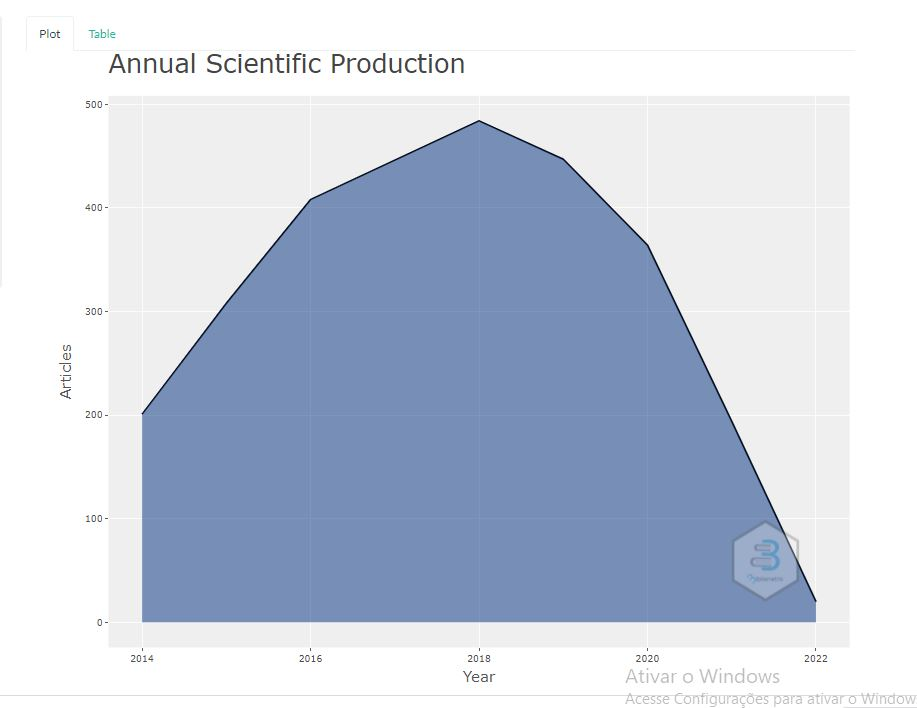
\includegraphics[width=1\textwidth]{experiments/guioliunb/AnaliseBibliometrica/SocialBigDataAnalysis/anual-scientific-production.JPG}
    \caption{Evolução da produção científica no \dataset\   SBDAA@guioliunb.}
    \label{fig:evol:anual:SBDAA@guioliunb}
\end{figure}

A figura \ref{fig:evol:anual:SBDAA@guioliunb} apresenta um declínio na produção mundial no tema de interesse, segundo o \dataset\  SBDAA@guioliunb. O ápice de produção foi alcançado no ano de 2018. Fica evidente que o ano de 2022 ainda não pode contribuir para a análise anual, pois ainda está em progresso.

\begin{figure}
    \centering
    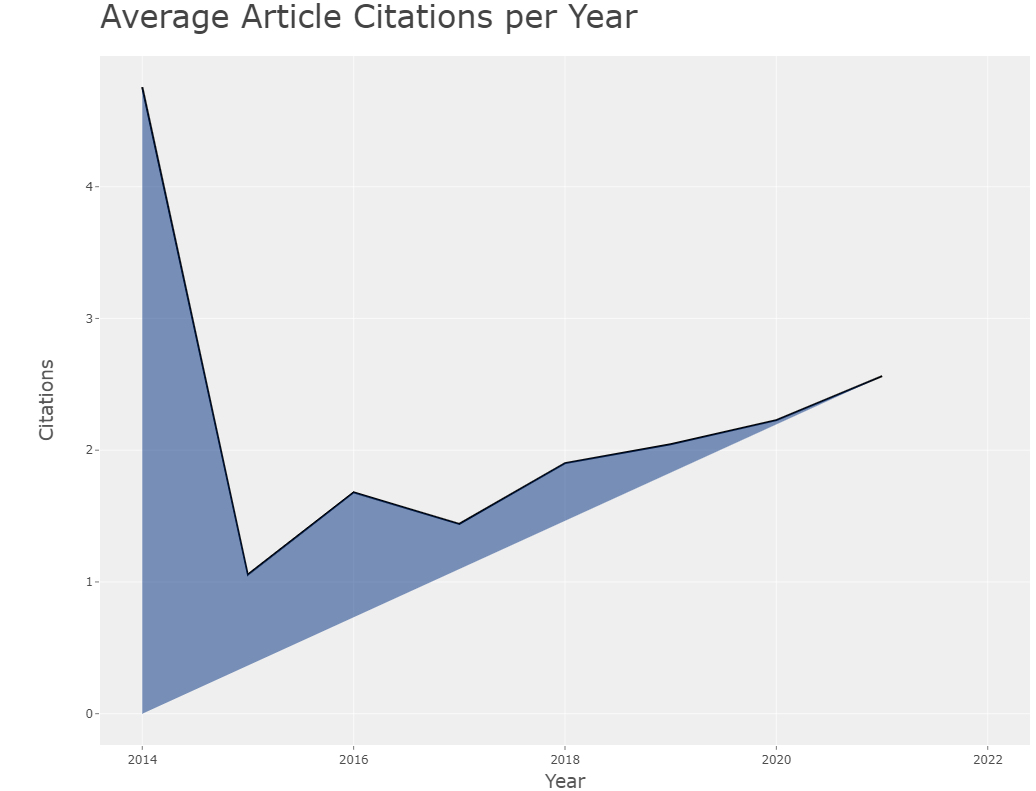
\includegraphics[width=1\textwidth]{experiments/guioliunb/AnaliseBibliometrica/SocialBigDataAnalysis/AVG citation per year.png}
    \caption{Evolução da produção científica no \dataset\   SBDAA@guioliunb.}
    \label{fig:evol:anual:cit:SBDAA@guioliunb}
\end{figure}




Já figura \ref{fig:evol:anual:cit:SBDAA@guioliunb} mostra que o número de citações é na verdade crescente. Então segundo o podemos questionar se o tema realmente está em declínio ou em dispersando entre outras bases e autores. Um fato comum após algum tempo da iniciação da pesquisa sobre alguma área é a ampliação do conhecimento, logo a distribuição também. Com a expressiva quantidade dos dados gerados nos desde 2018 é uma possibilidade considerar que os trabalhos podem ainda tenham crescido, porém diluídos em outros temas e profissionais.

\subsection{Interpretação do Crescimento} 

A taxa de crescimento anual teve o resultado negativo no, porém os últimos dois anos apresentou grande concentração de investimentos nas áreas de \textit{big data} e \textit{cloud computing}. Dado isso, podemos questionar se a área está em declínio ou outro motivo pode ter ocasionado isso na base adquirida.

\subsection{Evolução das Citações}

Somado a isso, temos a Figura \ref{fig:evol:anual:cit:SBDAA@guioliunb} que explicita que o uso do \dataset\  SBDAA@guioliunb em citações e estudos posterior é crescente. Logo, a produção de conteúdo e a evolução da área demonstra evolução e dispersão. Podendo assim responder o questionamento sobre o declínio da área.

Outro fato, é o acúmulo de citações por ano facilitando o gráfico continuar em uma crescente.



\subsection{Interpretação das Citações}
Com o crescimento das citações fica evidente o repetição do uso nos artigos e o ganho de relevância do \dataset\ diante o tempo. Dessa forma, os novos registros bibliográficos herdam conceitos produzidos por esse bibliografia. Assim, demonstrando crescimento do interesse pela comunidade científica e aceitação de outros profissionais. Ou seja, uma tendência positiva do material produzido.
O crescimento das citações junto ao declínio de produções similares pode significar também a evolução da área para novos desafios. Assim o material registrado não é mais produzido mas utilizado para novas produções de artigo.

\subsection{\textit{Three-Field Plots (Sankey diagram)} \label{SBDAA:Sankey}}

\begin{figure}
    \centering
    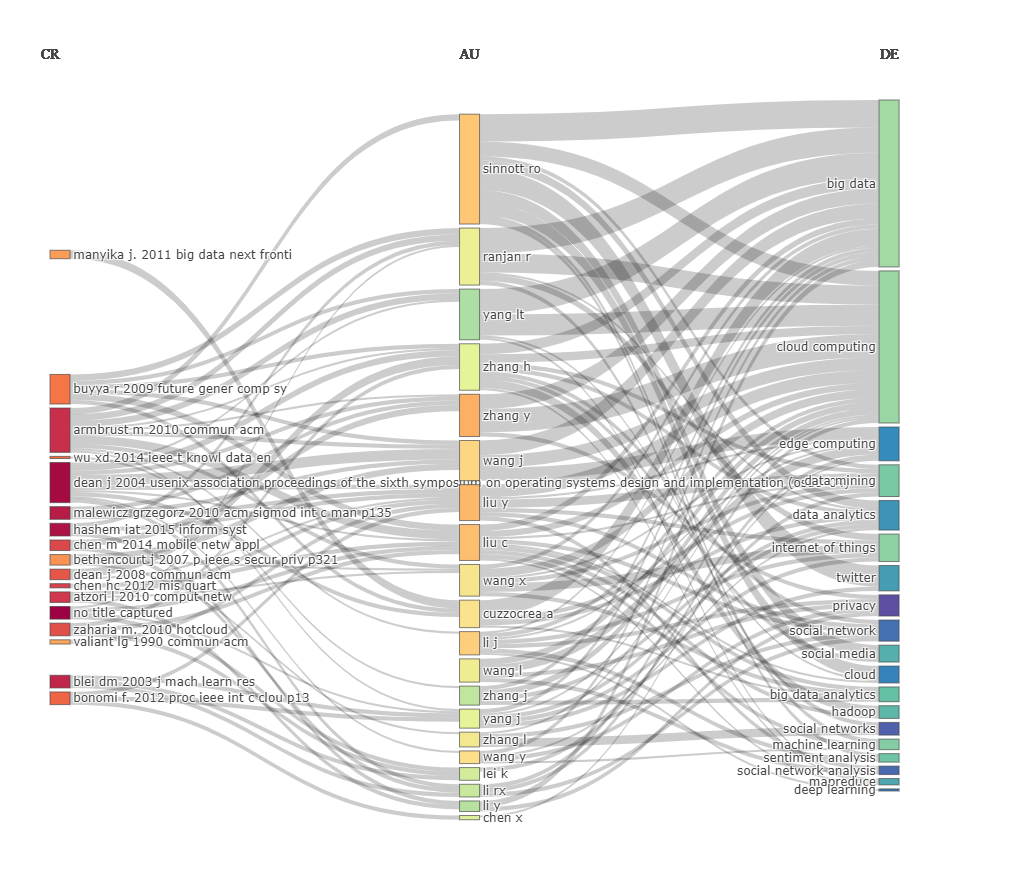
\includegraphics[angle=0,width=1\textwidth]{experiments/guioliunb/AnaliseBibliometrica/SocialBigDataAnalysis/3FSE-referencesXauthorsXkeywords.png}
    \caption{Plotagem ``Três Campos'' (Sankey plot) do \dataset\ SBDAA@guioliunb: Referências, Autores, e Palavras-Chave.}
    \label{fig:SBDAA@guioliunb:ThreeFieldPlot}
\end{figure}

As \textit{Three-Field Plots (Sankey diagram)} (plotagens do tipo ``Três Campos'') apresentam afinidades entre três conjuntos de atributos agregados que ocorrem no \dataset. Uma plotagem do tipo Sankey busca mostrar os principais fluxos entre diferentes conjuntos de itens. \footnote{Para uma introdução ver \url{https://en.wikipedia.org/wiki/Sankey_diagram}. Para obter detalhes sobre a forma de geração e utilização desse gráfico, inclusive de forma interativa, veja o vídeo em \url{https://www.youtube.com/watch?v=jBb1iha6-sg}.} 



A figura \ref{fig:SBDAA@guioliunb:ThreeFieldPlot} apresenta a plotagem do tipo ``Três Campos'' do \dataset\   SBDAA@guioliunb, vinculando, ao centro, os 20 Autores mais proeminentes (AU), à esquerda, as 20 Citações mais frequentes (CR - Cited Records), e à direita, as 20 Palavras-Chave mais frequentes empregadas pelos autores.

Já a figura \ref{fig:SBDAA@guioliunb:ThreeFieldPlot2} apresenta a plotagem do tipo ``Três Campos'' do \dataset\   SBDAA@guioliunb, vinculando, ao centro, os 20 Autores mais proeminentes (AU), à esquerda, os países de origem mais recorrentes , e à direita, os títulos com maior intersecção entre os artigos.



\begin{figure}
    \centering
    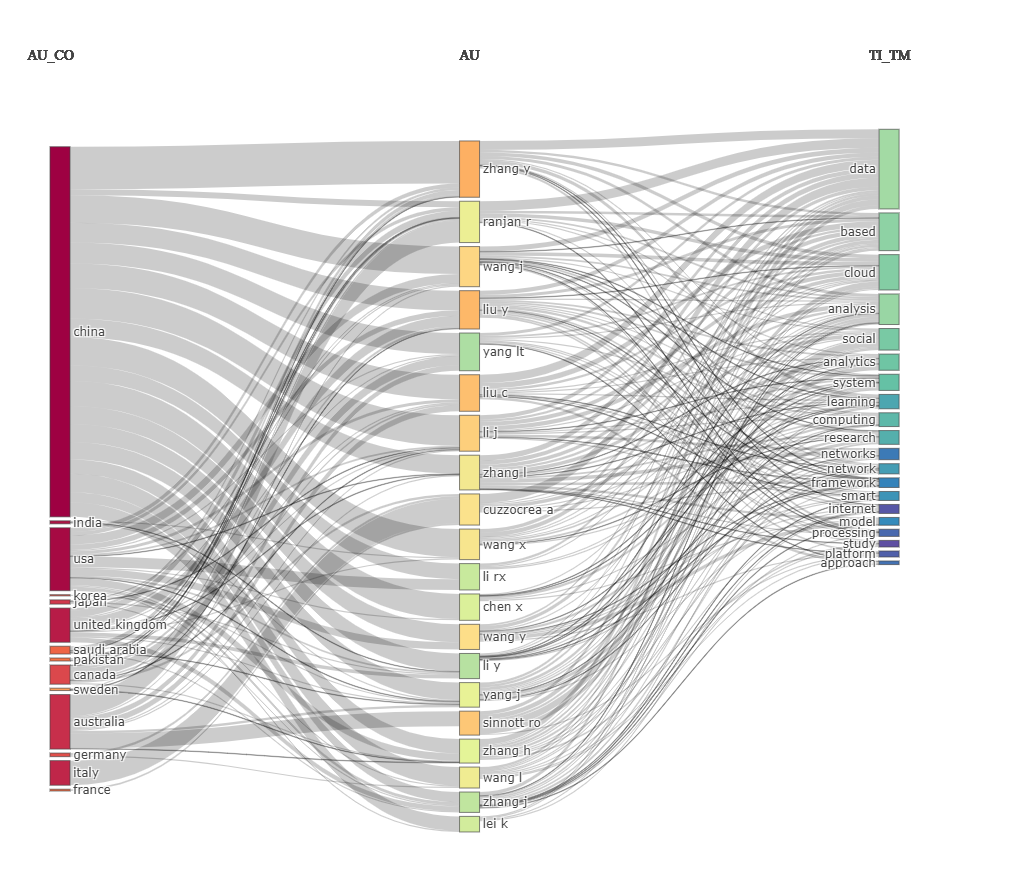
\includegraphics[angle=0,width=1\textwidth]{experiments/guioliunb/AnaliseBibliometrica/SocialBigDataAnalysis/3FSE-countriesXauthorsXtitles.png}
    \caption{Plotagem ``Três Campos'' (Sankey plot) do \dataset\   SBDAA@guioliunb: 20 Países, Autores e Títulos.}
    \label{fig:SBDAA@guioliunb:ThreeFieldPlot2}
\end{figure}

\subsection{Interpretação da figura \ref{fig:SBDAA@guioliunb:ThreeFieldPlot}}



A figura \ref{fig:SBDAA@guioliunb:ThreeFieldPlot} explicita uma rede de produção de conhecimento bem conectada entre os 20 autores, ou seja, são cientistas bem ativos no tema e trabalham em contribuição para um objetivo comum.

\textit{Big Data} e \textit{Cloud Computing} são as palavras-chaves com maior relevância fazendo jus à necessidade de integração entre as duas áreas na formação da base estudada.
Também, pode-se observar o surgimento de áreas relacionadas aos dois aspectos principais como: edge computing, data mining, data analytics e outros. Esses assuntos de fato são utilizados com as duas principais \textit{keywords}, então é interessante observar suas possíveis ramificações.
Além disso, os principais autores possuem um grande coeficiente de citações feitas e recebidas. Podendo assim ser um indicador de qualidade de seus trabalhos científicos.

\subsection{Interpretação da figura \ref{fig:SBDAA@guioliunb:ThreeFieldPlot2}}

Na segunda figura \ref{fig:SBDAA@guioliunb:ThreeFieldPlot2} é razoável  observar a grande contribuição da China no \dataset\ e consequentemente entender a grande participação dos chineses nos autores mais relevantes como mostrado na \ref{fig:SBDAA@guioliunb:ThreeFieldPlot}. Acrescentado com a contribuição chinesa fica também evidente uma porcentagem razoável de EUA e Austrália.

O termo mais utilizado nos títulos é \textit{data} concordando com as palavras-chaves anteriormente analisadas. As outras categorias tem um significado acoplado com o termo \textit{data}, pois ao observar os artigos formam: modelos, métodos, \textit{frameworks},\textit{networks} e sistemas especializados no uso de \textit{data}.


\subsubsection{Autores mais relevantes\label{MASSA:Sankey:AutoresRelevantes}}

A figura \ref{fig:SBDAA@guioliunb:relevantauthors} confirma uma grande participação chinesa nessa área de pesquisa. Porém, deve ser levado em conta a possibilidade de nomes homônimos ou participações do mesmo contribuidor com assinatura de sobrenome diferente nos trabalhos.

\begin{figure}
    \centering
    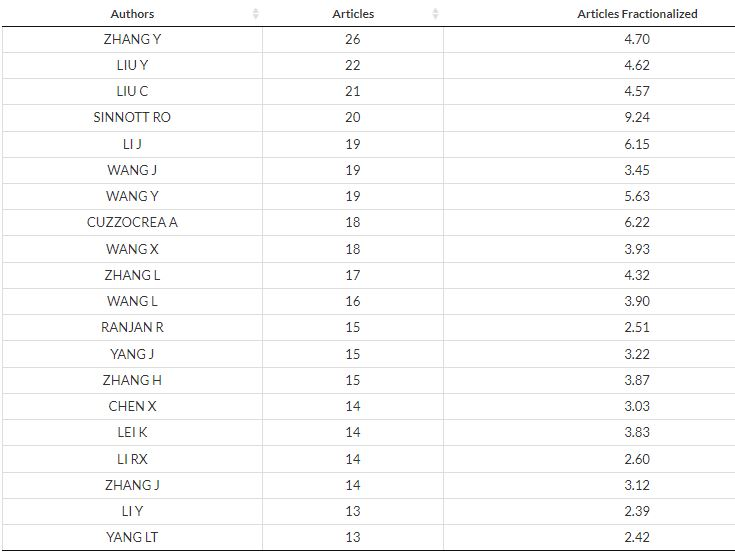
\includegraphics[angle=0,width=1\textwidth]{experiments/guioliunb/AnaliseBibliometrica/SocialBigDataAnalysis/most relevant authors.png}
    \caption{Autores mais relevantes do \dataset\   SBDAA@guioliunb.}
    \label{fig:SBDAA@guioliunb:relevantauthors}
\end{figure}


\subsection{Medidas bibliométricas}

As medidas bibliométricas propriamente ditas, relativas ao \dataset\ SBDAA@guioliunb, serão exploradas nesta subseção, e são organizadas em três conjuntos:
\begin{description}
    \item [Relativas às Fontes de Informação] Uma vez que foram consideradas apenas as publicações em revistas, todas as fontes de informação mensuradas serão revistas científicas, ou \textit{journals}. As principais medidas são de impacto das fontes, mensuradas com base no número de citações que os artigos publicados nas revistas obtiveram de outras publicações, possivelmente feitas em outras fontes de informação, como outras revistas, seções de livros, artigos de conferência etc. As citações são registradas pelas organizações que fazem indexação de artigos, como a Web of Science e SCOPUS;
    \item [Relativas aos Autores] Sempre que um artigo publicado por um ou mais autores e também indexado por uma organização (Web of Science,  SCOPUS etc), é citado em um outro artigo também indexado por essa mesma organização, então é feita a anotação de uma citação ao mesmo, e o impacto potencial desse autor sobre a ciência é atestado pelo valor mais alto da citação do conjunto de seus artigos indexados. Várias métricas (índice H, G, M etc) podem ser derivadas dessa medida (quantidade de citações), e são exploradas tanto em relação aos autores como em relação às revistas onde esses artigos foram publicados;
    \item [Relativas aos Documentos] Cada citação adicional a  um documento (artigo de revista, de conferência, livro, ou  capítulo de livro) é um indicador do impacto do documento em si, que evidencia a sua importância. Além das citações, a ocorrência de palavras dentro dos documentos, inclusive ordenada pelo tempo, também produz indicadores numéricos (métricas) relevantes para analisar a importância do documento em relação a outros. 
\end{description}

Essas medidas serão apresentadas a seguir.

\subsubsection{Bibliometrias aplicadas aos documentos (Artigos científicos) no \dataset}

\paragraph{Citações globais aos artigos no \dataset}

Cada registro recuperado possui nos seus metadados informações, podendo constar a quantidade de vezes que uma citação ao mesmo foi registrada no índice do WoS (\textit{TC - Times Cited}).
A figura \ref{fig:SBDAA@guioliunb:relevantdocuments} evidência as publicações mais referenciadas. Os 4 primeiros itens tem uma dominância considerável sobre os outros, contudo é interessante observar que são dois trabalhos com referências acopladas, pois o número e título do primeiro se assemelha muito ao segundo, assim como o terceiro se assemelha ao quarto. Como confirmação ambos código DOI são iguais par a par.

Os outros registros se comportam como registros individuais. Porém, vale ressaltar que uma relevante parte deles foi publicado na organização IEEE. A ordem de relevância das fontes será analisada em seção posterior.




\begin{figure}
    \centering
    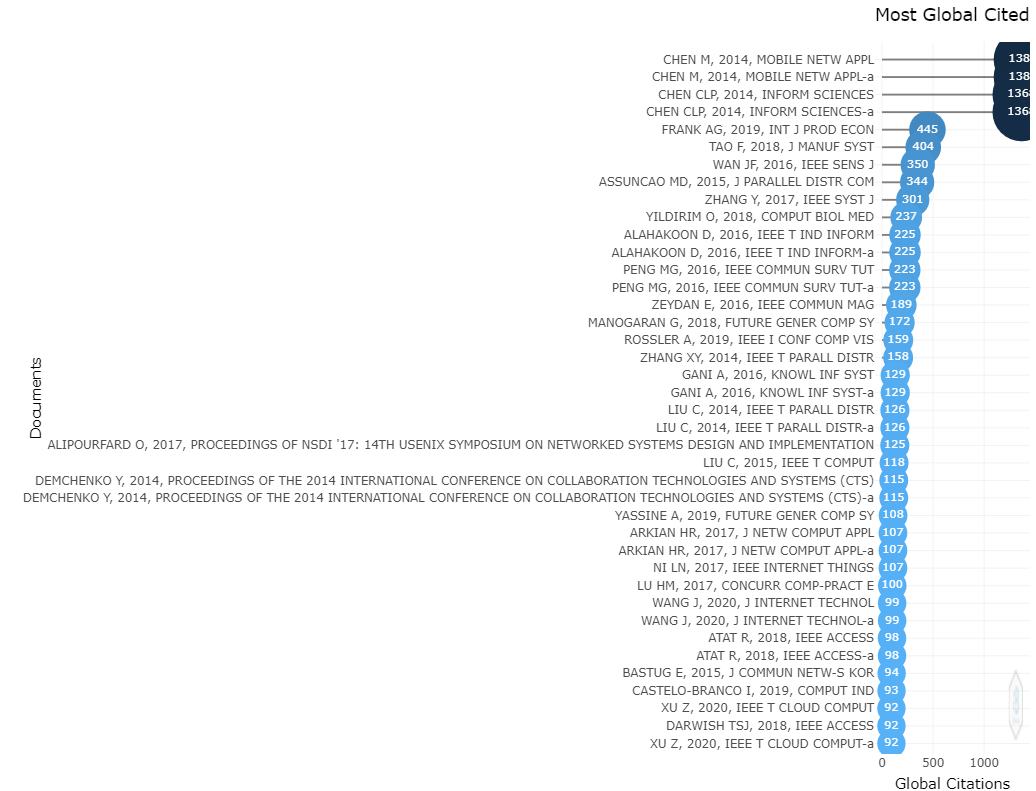
\includegraphics[angle=0,width=1\textwidth]{experiments/guioliunb/AnaliseBibliometrica/SocialBigDataAnalysis/MOST GLOBAL CITED.png}
    \caption{Autores mais relevantes do \dataset\ SBDAA@guioliunb no contexto global .}
    \label{fig:SBDAA@guioliunb:relevantdocuments}
\end{figure}

Após a visitação do resumo do texto de vários dos documentos citados, percebe-se que não refletem bem o foco do \dataset, o que se justifica pelo fato de que esses documentos são os de maior citação global, e não necessariamente os que tem maior citação local ao \dataset\. Dessa forma, procede-se à próxima análise.

\paragraph{Citações locais aos artigos no \dataset}

Podemos também visualizar as citações feitas apenas dentro do \dataset\. Com isso o mapeamento da relevância da citações pode ser observada internamente, ou seja, essa métrica pode auxiliar a identificação de publicações bem refinadas da consulta executada.  


\begin{figure}
    \centering
    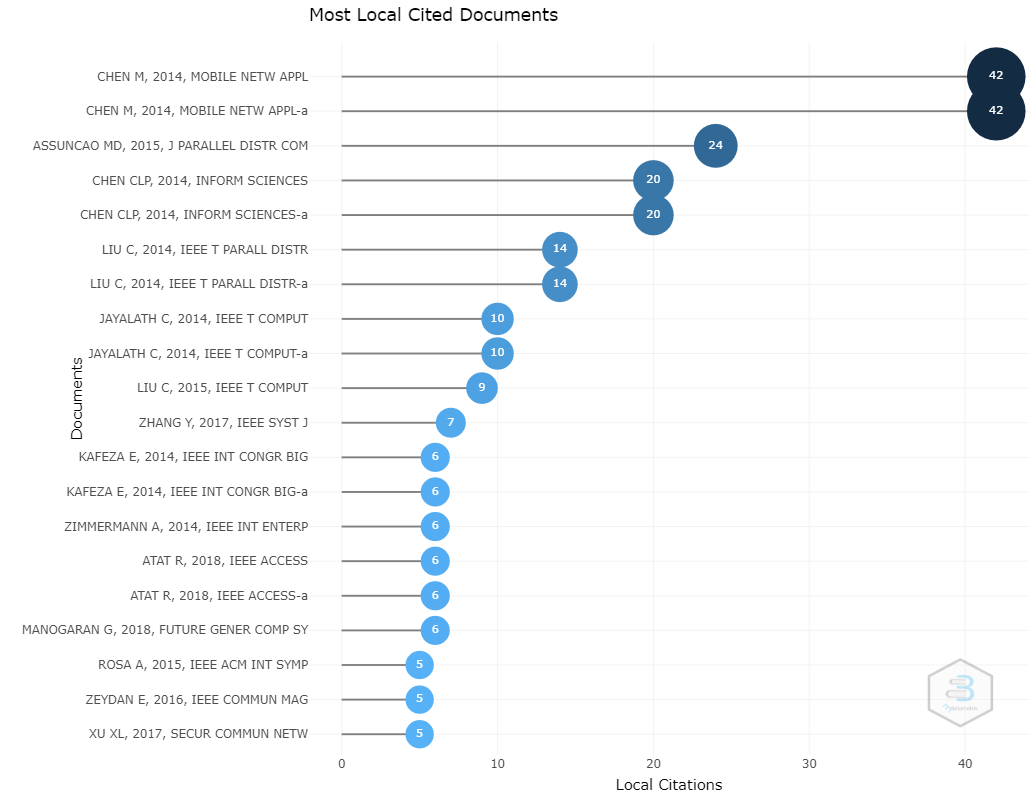
\includegraphics[angle=0,width=1\textwidth]{experiments/guioliunb/AnaliseBibliometrica/SocialBigDataAnalysis/MOST LOCAL CITED.png}
    \caption{Autores mais relevantes do \dataset\ no contexto local   SBDAA@guioliunb.}
    \label{fig:SBDAA@guioliunb:relevantdocuments}
\end{figure}


Após a apresentação das citações internas e externas da pesquisa feita resulta na coerência da relevância de grande parte dos trabalhos, já que sua participação é importante n \dataset\ e também para outros conjuntos de dados. Um registro que evidencia isso é o primeiro na ordem tanto global como local, demostrando uma contribuição importante para o estudo bibliomética sugerido.

\paragraph{Referências a outros documentos (artigos, capítulos de livros etc) citados pelos artigos no \dataset}

Ademais, é contabilizado as referências utilizadas pelos registros do \dataset\ SBDAA@guioliunb. Essa medida é um indicativo de boas fontes utilizada em comum para a produção dos artigos. Podendo assim serem utilizadas como fonte de conhecimento confiante, com aplicabilidade e em tendência de progresso.  

\begin{figure}
    \centering
    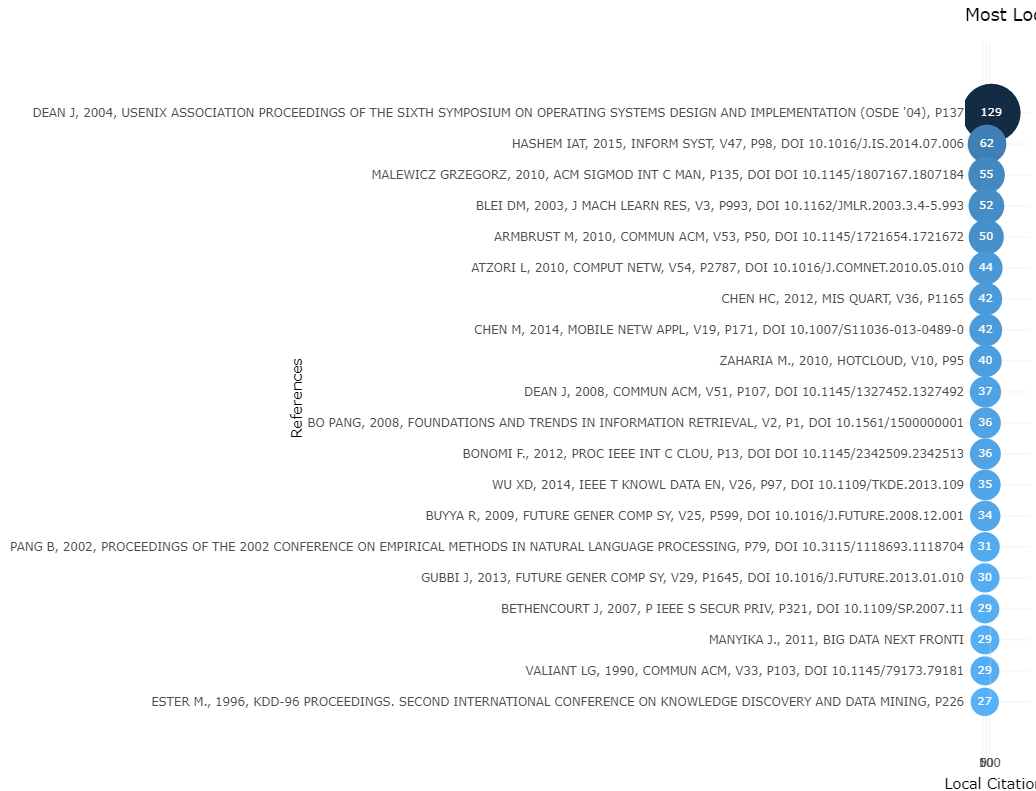
\includegraphics[angle=0,width=1\textwidth]{experiments/guioliunb/AnaliseBibliometrica/SocialBigDataAnalysis/MOST LOCAL CITED DOC.png}
    \caption{Referências mais relevantes do \dataset\ no contexto local   SBDAA@guioliunb.}
    \label{fig:SBDAA@guioliunb:relevantdocuments}
\end{figure}

\paragraph{Espectroscopia das referências}

A técnica de espectroscopia das referências bibliográficas (\textit{reference publication year spectroscopy}(RPYS)) de um \dataset \cite{marx_detecting_2014} possibilita identificar as raízes históricas de um campo de conhecimento. 

A figura \ref{fig:MASSA2-ReferenceSpectroscopy} apresenta o quantitativo de referências citadas pelo \dataset\, para cada ano.

\begin{figure}
    \centering
    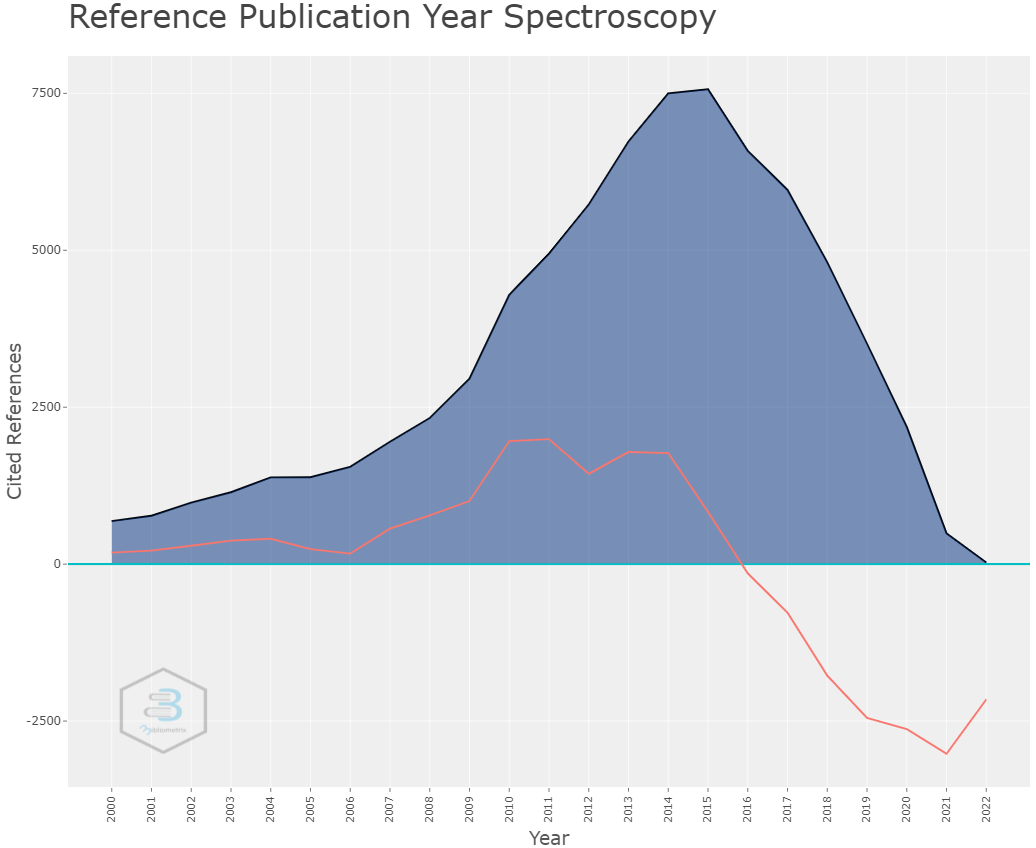
\includegraphics[width=1\textwidth]{experiments/guioliunb/AnaliseBibliometrica/SocialBigDataAnalysis/reference spectroscopy.png}
    \caption{Espectroscopia (RPYS) completa das referências do \dataset\ SBDAA@guioliunb.}
    \label{fig:MASSA2-ReferenceSpectroscopy}
\end{figure}

Através da espectroscopia fica coeso a redução do crescimento de publicações científicas anuais observado na \ref{fig:evol:anual:SBDAA@guioliunb}. Fato que faz sentido, afinal, com a diminuição das publicações é tendencioso que as citações diminuam.


\paragraph{Uso de palavras dentro dos artigos no \dataset}

É interessante também a demonstração dos termos mais frequentes na base de registros. Afinal, os tópicos mais frequentes são evidenciados, podendo assim apresentar algum padrão.
\ref{tab:MASSA2:Word:Occurrences}, com os 40 termos mais frequentes em uso.

\begin{figure}
    \centering
    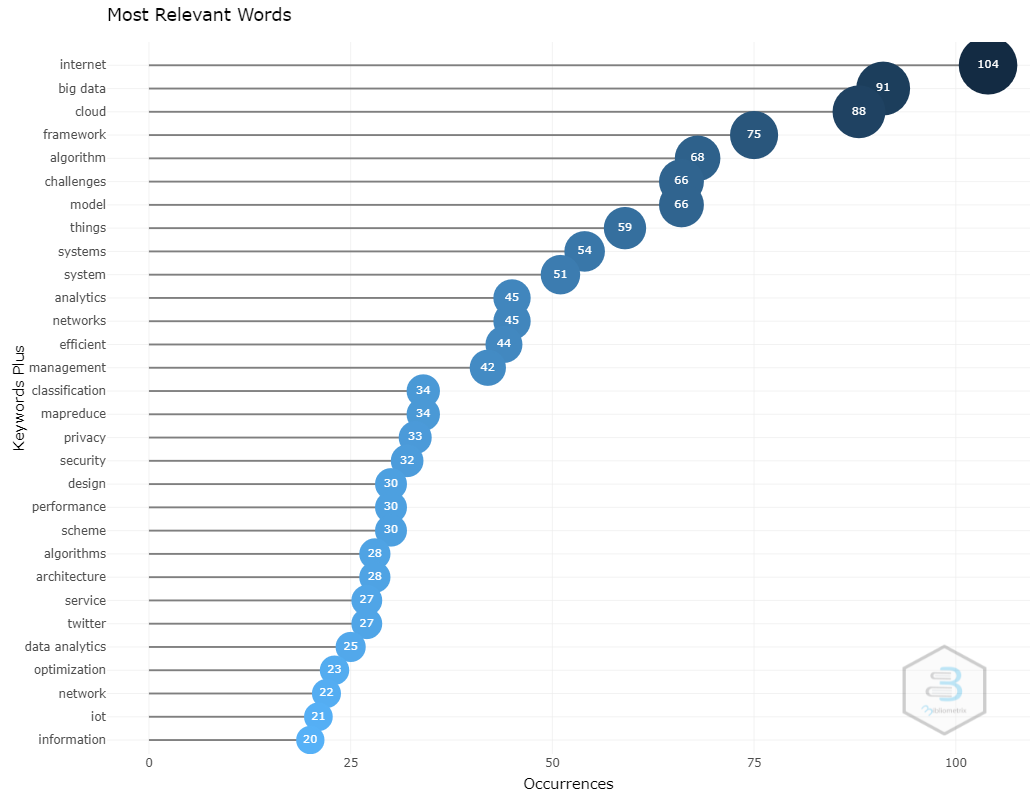
\includegraphics[width=1\textwidth]{experiments/guioliunb/AnaliseBibliometrica/SocialBigDataAnalysis/MOST FREQUENT WORDS.png}
    \caption{Termos mais frequentes no \dataset\ SBDAA@guioliunb.}
    \label{fig:MASSA2-ReferenceSpectroscopy}
\end{figure}

Além dessa podemos expor outra apresentação dos mesmos termos:
\begin{figure}
    \centering
    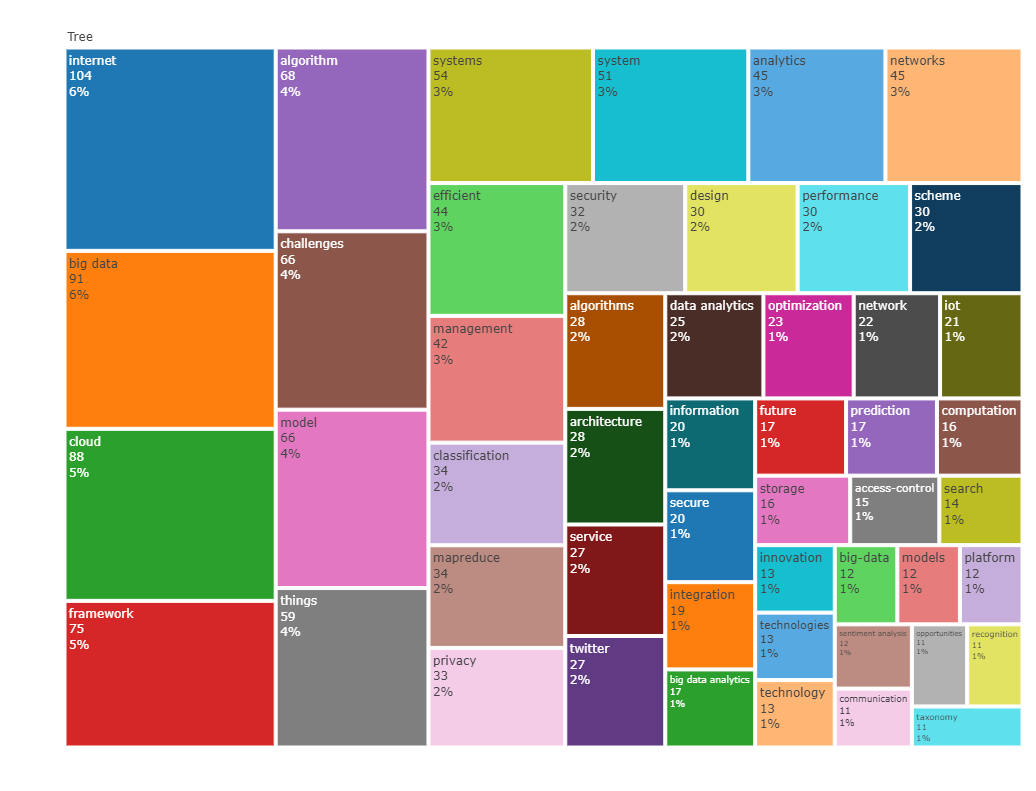
\includegraphics[width=1\textwidth]{experiments/guioliunb/AnaliseBibliometrica/SocialBigDataAnalysis/TREEMAP.png}
    \caption{Termos mais frequentes no \dataset\ com representação \textit{TreeMap} SBDAA@guioliunb.}
    \label{fig:MASSA2-TREEMAP}
\end{figure}


Por fim, o Bibliometrix permite apresentar o uso dos termos ordenado temporalmente:
\begin{figure}
    \centering
    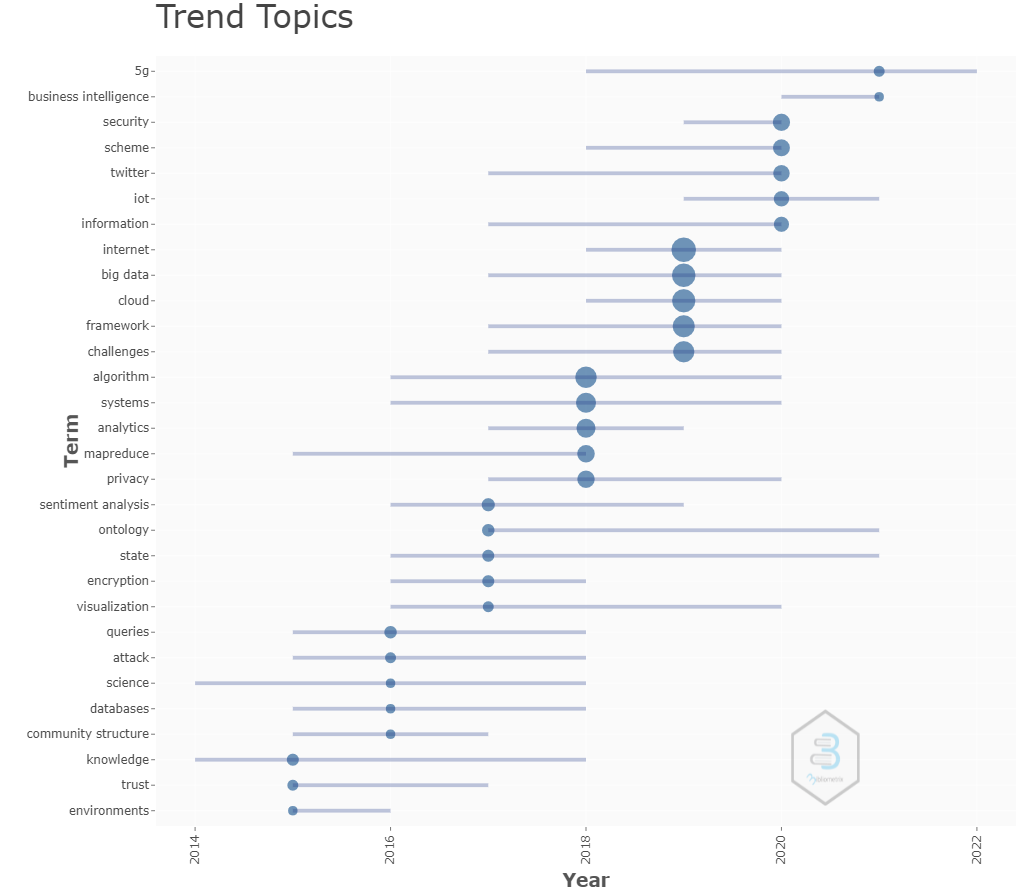
\includegraphics[width=1\textwidth]{experiments/guioliunb/AnaliseBibliometrica/SocialBigDataAnalysis/TREND TOPICS.png}
    \caption{Trend Topics no \dataset\ SBDAA@guioliunb.}
    \label{fig:trend:topics}
\end{figure}

Fato interessante na figura \ref{fig:trend:topics} é o surgimento dos termo: \texttt{5G}, \textit{security}, \textit{encryption}, \textit{privacy}, \textit{sentiment analysis} entre outros. Pois, são assuntos evidentes nos dias de hoje, em síntese ganharam relevância juntamente aos tópicos pesquisados.
Como também é confirmado as palavras-chaves do \dataset\ com a reincidência nos \textit{trend topics}, como em outras métricas.


\subsection{Métricas para Autores}

Como as contribuições científicas são frutos de trabalhos em conjunto é importante evidenciar aqueles que contribuíram para as facilidades que foram adquiridas e que estão sendo progredidas. Segue os gráficos de produção segundo tempo.


\begin{figure}
    \centering
    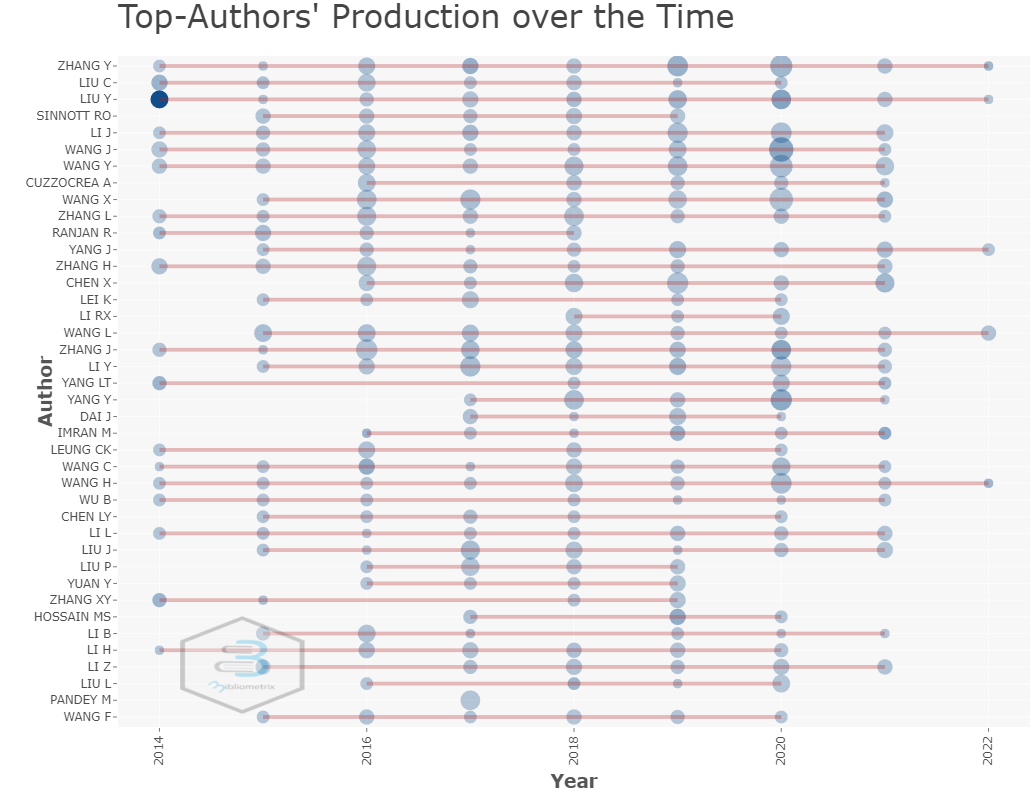
\includegraphics[width=1\textwidth]{experiments/guioliunb/AnaliseBibliometrica/SocialBigDataAnalysis/PRODUCTION OVER THE TIME.png}
    \caption{Autores mais produtivos \dataset\ SBDAA@guioliunb.}
    \label{fig:authors:production}
\end{figure}



\subsubsection{Autores mais relevantes localmente citados}

Além do mais podemos citar os autores com mais citações locais do no \dataset\ SBDAA@guioliunb.

\begin{figure}
    \centering
    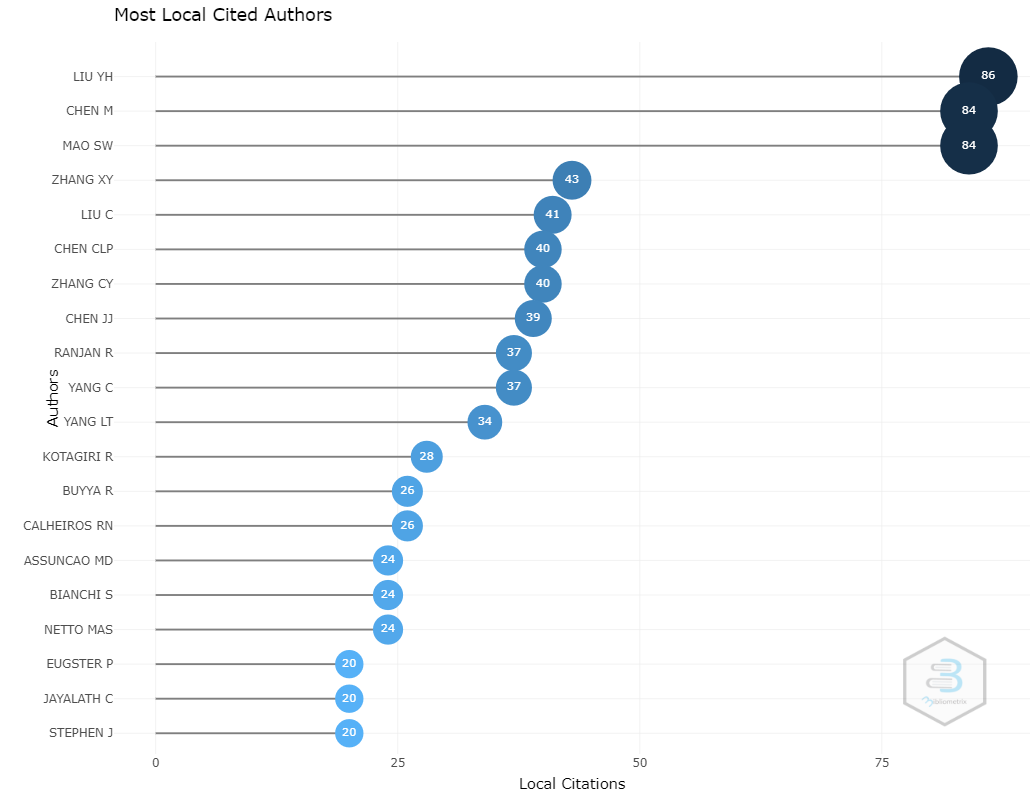
\includegraphics[width=1\textwidth]{experiments/guioliunb/AnaliseBibliometrica/SocialBigDataAnalysis/MOST LOAL CITED AUTHORS.png}
    \caption{Autores mais citados do \dataset\ SBDAA@guioliunb no contexto local.}
    \label{fig:authors:production}
\end{figure}


\subsection{Métricas para Fontes de Informação}

As métricas para fontes de informação permitem avaliar a qualidade das revistas, conferências, em relação ao impacto de publicações em determinado tema. Valem a maioria das medidas já vistas para autores.

\subsubsection{Fontes mais relevantes, conforme número de artigos publicados sobre o tema}

\begin{figure}
    \centering
    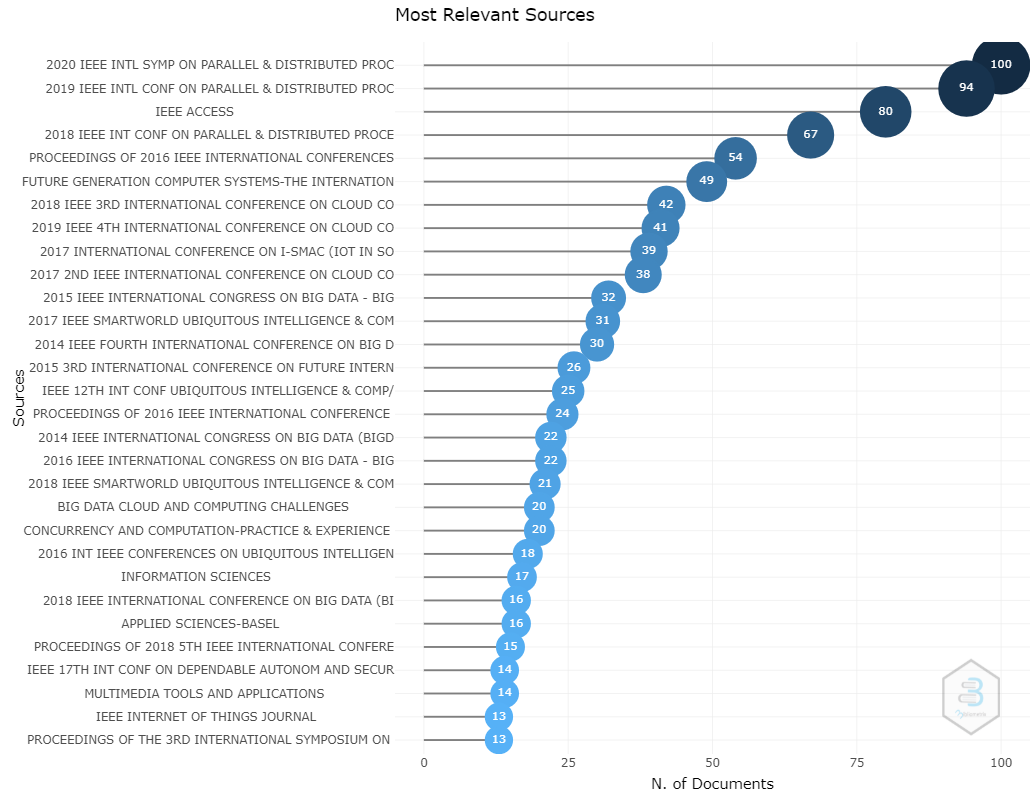
\includegraphics[width=1\textwidth]{experiments/guioliunb/AnaliseBibliometrica/SocialBigDataAnalysis/most relevant sources.png }
    \caption{Revistas mais relevantes no  \dataset\ SBDAA@guioliunb.}
    \label{fig:MASSA2-Most-Relevant-Sources}
\end{figure}



\subsubsection{Lei de Bradford}





\begin{figure}
    \centering
    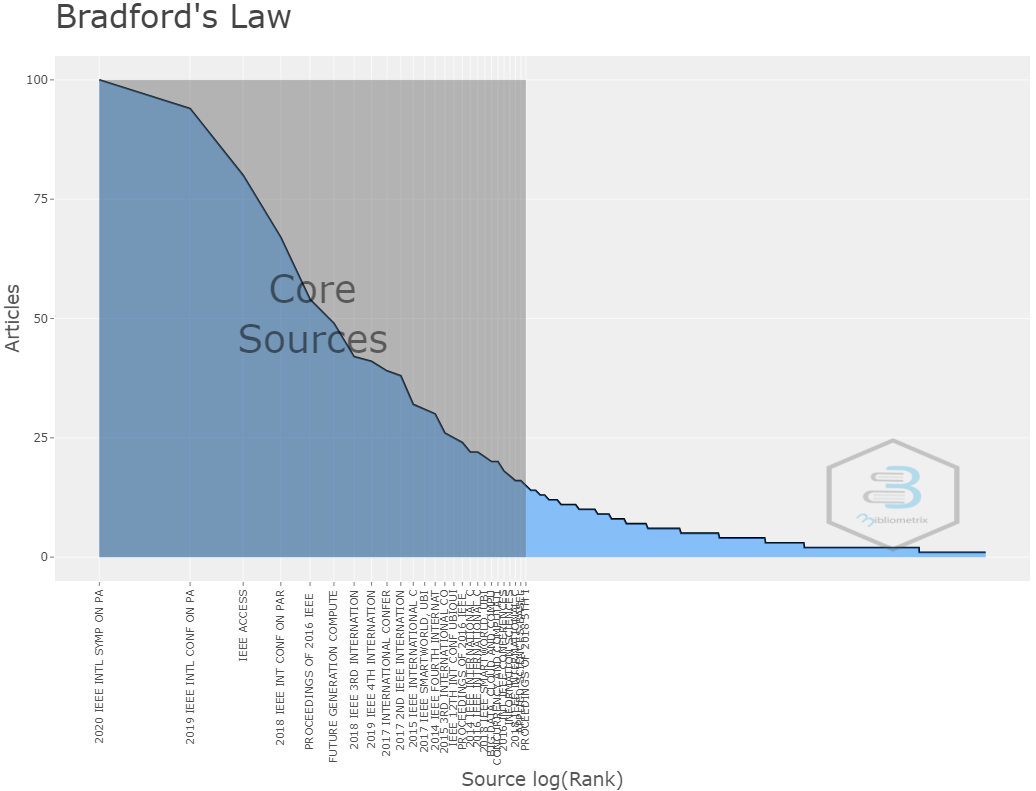
\includegraphics[width=1\textwidth]{experiments/guioliunb/AnaliseBibliometrica/SocialBigDataAnalysis/BRADFORDS LAW.png}
    \caption{Revistas mais relevantes no  \dataset\ SBDAA@guioliunb, conforme a Lei de Bradford.}
    \label{fig:MASSA2-Bradfords-Law.png}
\end{figure}


\subsection{Estrutura Conceitual do Conhecimento}

O Conhecimento científico é um fenômeno complexo que emerge a partir da agregação memética de termos e palavras, que representam conceitos e ideias, que se organizam em tópicos, temas, e que evoluem ao longo do tempo (ver \url{https://en.wikipedia.org/wiki/Memetics}).

A estrutura conceitual do conhecimento pode ser produzida pela análise de relacionamento estabelecidos entre esses termos. O bibliometrix apresenta um conjunto de técnicas para evidenciar essa estrutura conceitual, e que se organizam em dois grupos:
\begin{description}
    \item [Métricas em rede] que usam grafos para representar relacionamentos entre termos, evidenciando, por meio de métricas de análise de redes sociais, como o conhecimento conceitualmente se organiza.
    \item [Análise Fatorial] Que emprega métricas de redução da dimensionalidade, para explorar, usualmente em mapas bidimensionais, como os termos e palavras se relacionam. 
\end{description}

\subsubsection{Métricas aplicadas a grafos (redes)}

\paragraph{Redes de Coocorrências}

As redes de coocorrências apresentam importantes padrões que se formam nas publicações, e podem revelar a estrutura conceitual de uma área do conhecimento.

No Biblioshiny quatro tipos de redes coocorrências podem ser geradas:
\begin{itemize}
    \item Baseadas na coocorrência de termos, revelando quais são os termos mais comumente citados 
\end{itemize}

\begin{figure}
    \centering
    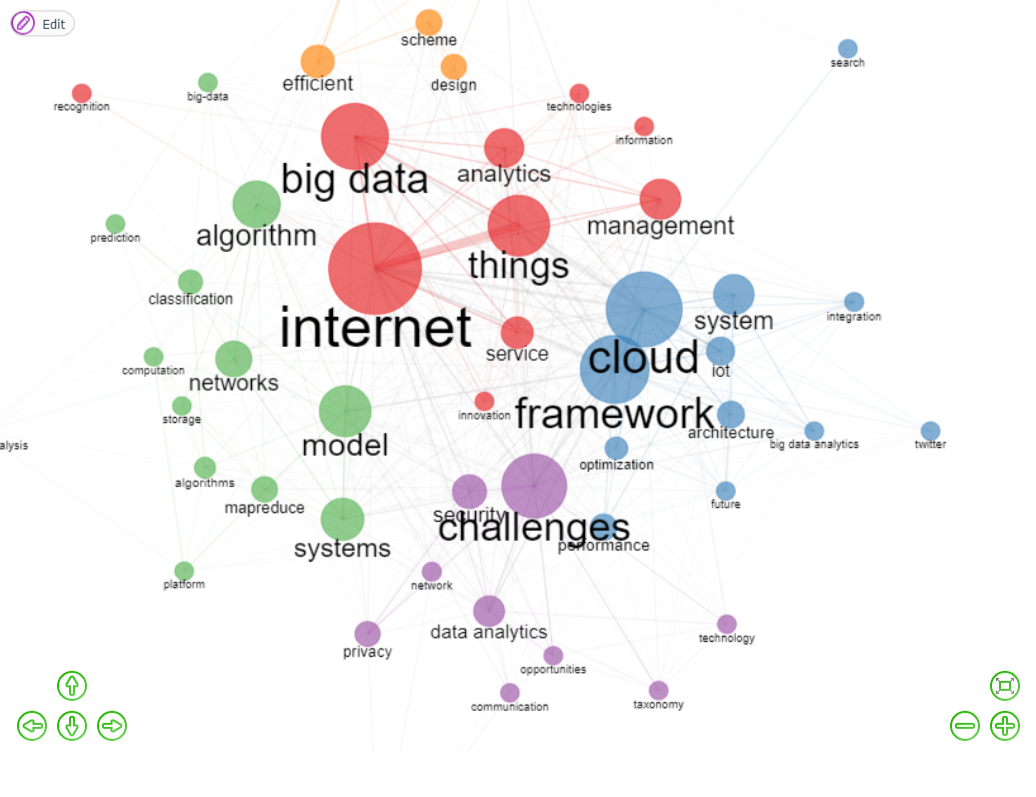
\includegraphics[width=1\textwidth]{experiments/guioliunb/AnaliseBibliometrica/SocialBigDataAnalysis/CO OCCURRRENCE NETWORK.png}
    \caption{Redes de Coocorrências no  \dataset\ SBDAA@guioliunb, conforme a Lei de Bradford.}
    \label{fig:MASSA2-Bradfords-Law.png}
\end{figure}



\subsubsection{Métricas de redução da dimensionalidade (Análise Fatorial)}

\begin{figure}
    \centering
    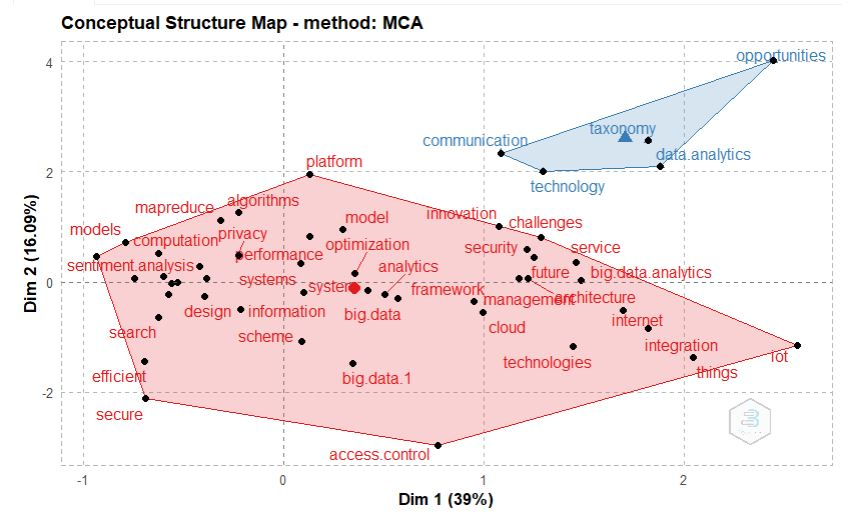
\includegraphics[width=1\textwidth]{experiments/guioliunb/AnaliseBibliometrica/SocialBigDataAnalysis/conceptual factorial.JPG}
    \caption{Dimensões de variabilidade mais relevantes, nas palavras-chave do  \dataset\ SBDAA@guioliunb.}
    \label{fig:MASSA2-FactorialAnalysis-MCA-FactorialMap}
\end{figure}


\subsection{Estrutura Intelectual  do Conhecimento}

Conhecimento científico é produzido por processos intelectuais onde autores de trabalho escolhem deliberadamente referenciar trabalhos de outros, por meio de documentos publicados, que são encaminhados para publicações em fontes de informação de sua escolha, e que evoluem ao longo do tempo.

O Bibliometrix permite exploração da estrutura intelectual do conhecimento, usando basicamente duas abordagens:
\begin{itemize}
    \item Redes de Co-Citação, abordagem bastante comum;
    \item Historiografia, abordagem pouco usual.
\end{itemize}

\subsubsection{Redes de Co-Citação}

\begin{figure}
    \centering
    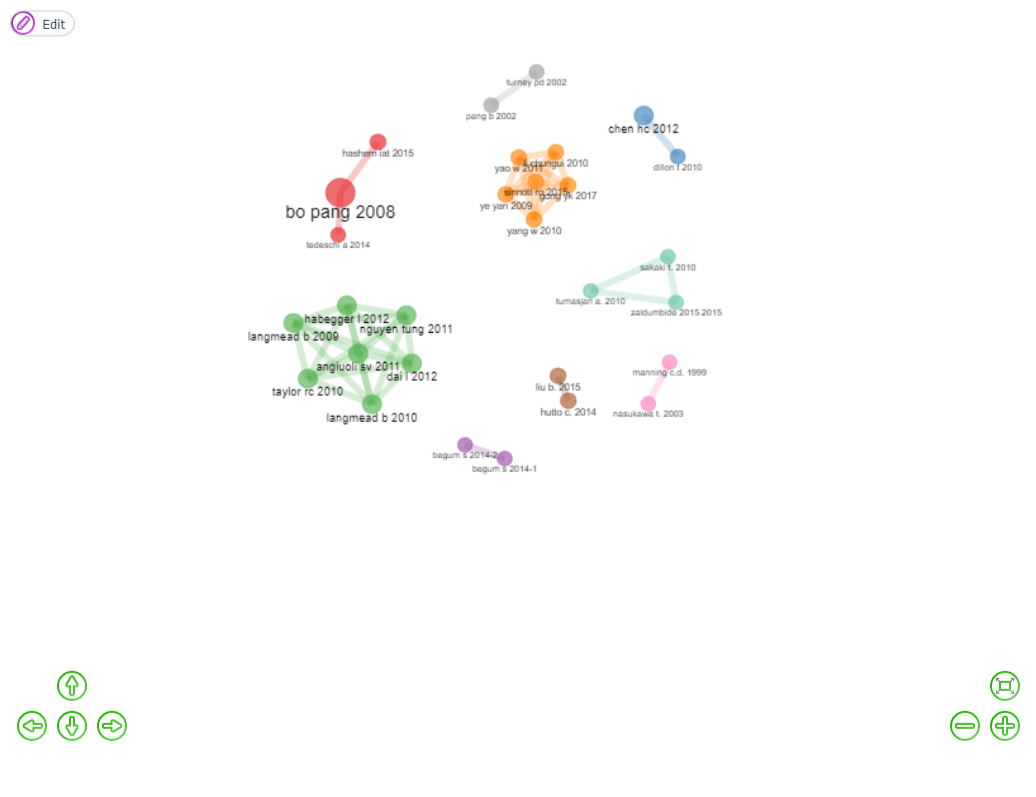
\includegraphics[width=1\textwidth]{experiments/guioliunb/AnaliseBibliometrica/SocialBigDataAnalysis/CO CITATION NETWORK.png}
    \caption{Rede de cocitação entre as referências mais presentes no  \dataset\ SBDAA@guioliunb.}
    \label{fig:MASSA2-CoCitation-Network}
\end{figure}

\subsubsection{Historiografia}






\begin{figure}
    \centering
    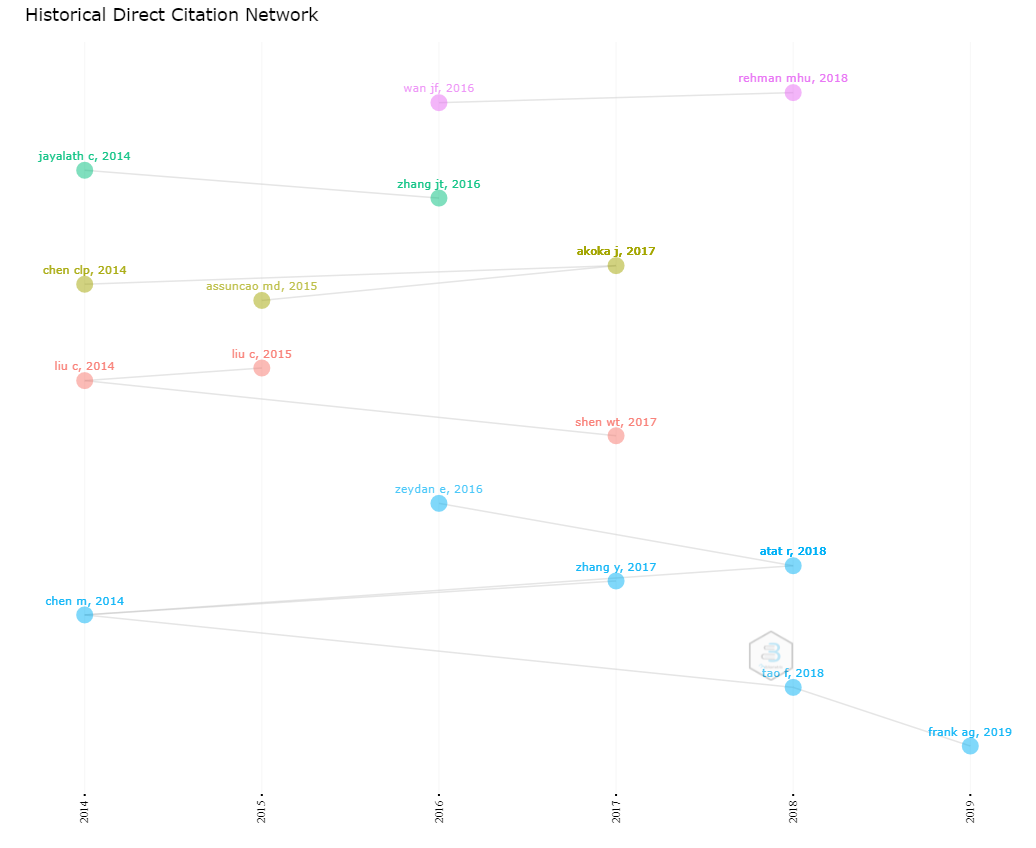
\includegraphics[width=1\textwidth]{experiments/guioliunb/AnaliseBibliometrica/SocialBigDataAnalysis/historiograph.png}
    \caption{Mapa histórico das citações diretas entre os documentos mais evidentes no  \dataset\ SBDAA@guioliunb.}
    \label{fig:MASSA2-HistoricalDirectCitationNetwork-100docs}
\end{figure}




\subsection{Estrutura Social do Conhecimento}

Conhecimento científico é produzido socialmente, por meio de autores trabalhando em conjunto, e uma estrutura de filiações a organizações permanentes ou periódicas, que realizam ou promovem pesquisas, nelas incluídos os centros de pesquisa, universidades, departamentos, institutos, faculdades, eventos, revistas, conferências, e que evoluem ao longo do tempo. A análise da estrutura social do conhecimento evidencia esses relacionamentos, que iniciam no plano pessoal, e evoluem para outros escopos.

\subsubsection{Rede de Colaboração}






\begin{figure}
    \centering
    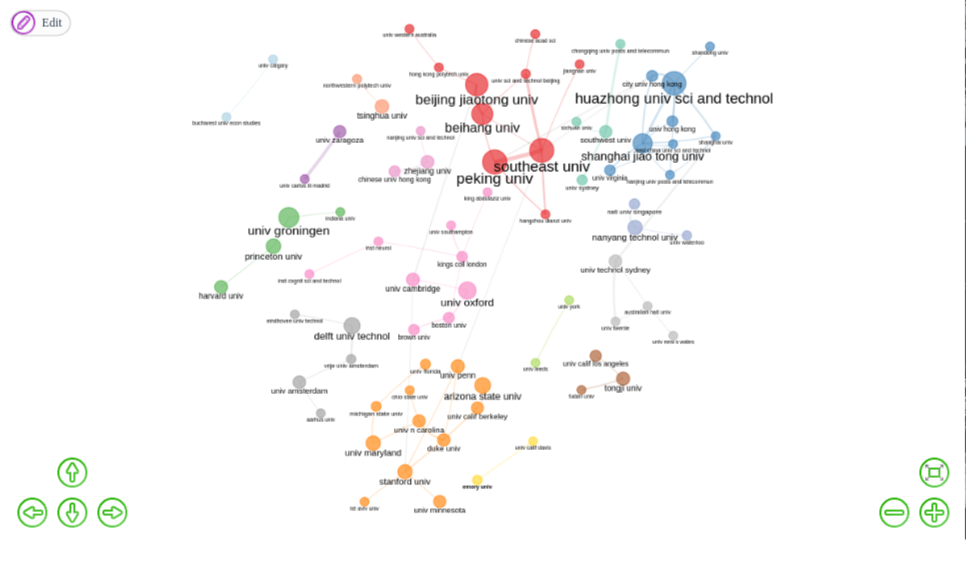
\includegraphics[width=1\textwidth]{experiments/jhcf/PesqBibliogr/SimulacaoMultiagente/WoS-20220203/Estrutura/Social/MASSA2-Collaboration-Network-150instit.png}
    \caption{Rede de colaboração entre as 150 instituições mais evidentes, no  \dataset\ SBDAA@guioliunb.}
    \label{fig:MASSA2-Collaboration-Network-150instit}
\end{figure}


\section{Análises\label{MASSA2:Analises}}

A pesquisa sobre análises de dados via nuvem é logicamente depende da evolução das áreas de \textit{Big Data} e \textit{Cloud Computing}. Porém fica evidente as grandes oportunidades de ramificação diante a junção dessas duas áreas. Podendo assim impactar a sociedade em diversas áreas como: saúde, segurança e eficiência de diversos processos que podem ser reproduzidos por máquina.

Sobre o \dataset\ analisado fica evidente uma base sólida e que se propagou diante novas publicações pela consistência de referências adquiridas. Além disso, os registros analisados trouxeram uma situação de proporcionalidade real sobre os termos de ascensão atuais, até mesmo sobre as tecnologias que são desafios.

Todavia, é notável uma concentração alta da produção desse conhecimento. Muito presente em alguns países e autores principais, nem sempre presente com relevância em um âmbito global.

As análises representaram bem as redes de colaboração, bem como as redes de termos que compõe o principais tópicos pesquisados. Fica evidente as organizações com grande esforço nessa área através das análises de fontes. Somado a isso, obteve-se um material referencial com aprovação científica, dessa forma podendo servir para estudos futuros.

\section{Conclusões}

Enfim, a bibliometria gerada trouxe boas conclusões sobre o assunto, até mesmo confirmações de tendências já conhecidas. Em suma, o material bibliográfico pesquisado foi bem mapeado segundo publicações e autores.

Também, através dos resultados obtidos podemos concluir que os dados são coerente sobre diferentes métodos, ou então os resultados certamente mostrariam algum desvio.

Um bom avanço foi obtido nas análises de dados. Ainda que possa ser continuado o trabalho de análise com a agregação de novos registros relevantes para mapear o tópico estudo. Assim como a melhora dos dados que contribuam melhor para a pesquisa, através de exclusão de possíveis registros incoerentes. Também é possível adicionar novas teorias não presente no documento que podem auxiliar na tomada de novas conclusões.

Grandes esclarecimentos sobre as ferramentas de trabalho e maior domínio na competência de bibliometria foi alcançado. Portanto, o trabalho foi realizado com êxito e sua proposta de entendimento foi de grande parte alcançada.

